\chapter{Traffic Light Prediction}\label{ch:prediction}

 \section{Introduction}

The lack of awareness among road users about the planned switching of traffic lights leads to a series of well-known problems. Firstly, the issue of unneeded stopping and idling at red lights unnecessarily increases energy expenditure and emissions. In addition, not knowing about the upcoming traffic light's switching behavior also has negative impacts on road safety. There is a so-called dilemma zone when approaching a traffic light, where it unexpectedly turns yellow, and one must decide whether to stop before the light \cite{zhang_yellow_2014}. Often, this can lead to running a red light, speeding, or misunderstandings between drivers, increasing the overall risk of accidents.

Such situations exemplify where improved communication between vehicles and infrastructure elements could reduce the risk of accidents and the inefficiency of traffic. Collaborative awareness is a key driver in current research on Cooperative Intelligent Transport Systems (C-ITS). Predicting traffic lights and communicating this prediction to vehicles, establishing the C-ITS day-1 service GLOSA, is one integral part of a larger portfolio of potential measures \cite{mellegard_day_2020}. Nonetheless, it is important to consider that traffic light prediction is not strictly limited to GLOSA-like systems and may also lay the foundation for other application scenarios. Especially with the emergence of Augmented Reality, there may be many more application scenarios than we currently envision.

Despite these encouraging prospects, traffic light prediction is currently associated with multiple challenges. When intuitively considering the topic, one might assume that predicting the switching behavior of a traffic light should be straightforward based on its control program. In fact, the deployment of countdown displays at traffic lights based on these control programs is widespread, especially in Asian areas \cite{pan_impact_2023} and has recently also been studied for cyclists \cite{kaths_green_2019}. However, these countdown displays operate by transferring the residual phase time directly within the control unit to a countdown controller \cite{islam_improved_2016}. A mobile system would need to access this information from the outside.

Hence, a mobile system working across multiple intersections requires an interoperable data source. Here, the option exists to obtain the control programs directly, but without the current internal program state \cite{zweck_traffic_2013}. Since traffic-adaptive signals may only decide a few seconds before the next cycle how long the green phase will be switched \cite{islam_improved_2016}, this method is restricted to fixed-time traffic light control programs \cite{zweck_traffic_2013}. However, only 161 out of 1731 intersection nodes in Hamburg run a fixed-time program as of 2023. As seen in \Cref{tab:control-programs}, another factor hindering a prediction based on the engineering plans of control programs is the large variety of formats, in addition to the limited availability.

\begin{table}[htbp]
    \centering
    \begin{tabular}{lr}
        \hline
        \textbf{Control Method} & \textbf{\# Intersections} \\
        \hline
        \multicolumn{2}{l}{\textit{Adaptive Traffic Light Control Programs}} \\
        COMTESS* & 61 \\
        FLUSS* & 2 \\
        VS-PLUS* & 53 \\
        TELAN/TRENDS* & 14 \\
        Open Method of Traffic Control (OMTC) & 738  \\
        Switching based on request & 702 \\
        \hline
        \multicolumn{2}{l}{\textit{Non-Adaptive Traffic Light Control Programs}} \\
        Fixed-time (with audible signals for visually impaired people) & 69 \\
        Fixed-time (without audible signals for visually impaired people) & 92 \\
        \hline
        \multicolumn{2}{l}{\footnotesize{*: Gradually being replaced by OMTC.}}
    \end{tabular}
    \caption{Traffic control methods at intersections in Hamburg\footnotemark{}.}
    \label{tab:control-programs}
\end{table}

Due to these issues, another method for traffic light prediction has been established to deploy GLOSA-like applications in the field. Most GLOSA applications make use of the residual time provided by Signal Phase and Timing (SPaT) messages generated on the intersection controller level and transmitted to the vehicle. However, such messages may not always be available at the given location -- sometimes, as in this work, the prediction of traffic lights has to be performed purely by observing the outside state. In this chapter, we will discuss the various methods for obtaining traffic light state information and evaluate which methods are practical for cyclists.

One issue we will investigate in more detail is the traffic-adaptiveness of the switching programs. Traffic-adaptive adjustments of switching programs are intended to improve the traffic flow at an intersection but have adverse effects on predictability due to short-term green time adjustments. This means that a prediction based on historical data may not always be accurate to the second. Furthermore, a challenge when deploying a prediction algorithm is that traffic light data may not always arrive complete or on time, which is particularly problematic when the prediction needs to adapt quickly to a short-term change. Hence, tolerance for errors and robustness against missing information are also of high importance. If the prediction is unavailable or inaccurate, it can quickly lead to a loss of trust for the user or even become a safety risk.

\footnotetext{Source: Traffic control inventory of the LSBG / IVS1 (as of June 22, 2023) provided on request, in addition to an inquiry to the Hamburg senate. See \url{https://www.buergerschaft-hh.de/parldok/dokument/72143/ampelschaltsysteme_gruene_welle.pdf}}

The goals of this chapter are as follows. First, we will investigate potential sources of real-time traffic light data and evaluate their practicality for cyclist applications. Afterward, we will review approaches that address traffic-adaptive timing in traffic light predictions. Combining learnings from both domains, we establish methods for a traffic-light prediction infrastructure for Hamburg. Based on a broad analysis of the adaptivity seen in the real-time data, we will study at how many intersections a prediction could be challenging. This study allows us to draw conclusions about the suitability of our chosen prediction method. Finally, we evaluate the accuracy, availability, and scalability of the prediction algorithm over a time span of one year.

\section{Related Work}

Related work has been conducted on overcoming issues in obtaining traffic light data and predicting traffic lights based on that data. For data acquisition, decentralized and centralized systems have been proposed and studied. Largely independent of these studies, multiple prediction methods that aim to improve prediction accuracy have been proposed. However, a holistic approach to traffic light prediction requires interleaving both perspectives, considering that the prediction method is influenced by the technical constraints the data acquisition system imposes. Learnings from both domains must be joined to develop a state-of-the-art prediction system.

\subsection{Decentralized Systems}

In Europe, a large body of research and investments is flowing toward decentralized traffic light data systems, especially those based on Dedicated Short-Range Communication (DSRC). To operate these systems, Road Side Units (RSUs) are deployed at intersections where they send out standardized radio messages on the 5.9 GHz frequency band. These standardized C-ITS messages include SPaT messages, which vehicles can directly collect with a corresponding antenna (On Board Unit, OBU). An SPaT message contains not only the current switching state of a traffic light but also a residual time until the next switch, making it an ideal data foundation for GLOSA applications. Thus, many studies related to GLOSA utilize this data foundation \cite{schweiger_elisatm_2011, rakha_eco-driving_2011, rakha_aeris_2012, li_open_2012, suramardhana_driver-centric_2014, xu_bb_2015, bernais_design_2016, nguyen_efficient_2016, choudhury_integrated_2016, stahlmann_multi-hop_2017, stahlmann_exploring_2018, plianos_predictive_2018, zhang_green_2020, chen_developing_2022}.

SPaT messages are typically generated within the intersection controller level \cite{zweck_traffic_2013} and transmitted directly to an RSU without the need for a centralized server system. However, such a system is typically not fully decentralized. To calculate the residual time, there is the need for an additional prediction module, which may communicate with its own cloud in which a prediction algorithm is running \cite{strobl_c-its_2019, neuner_leitfaden_2020}. Due to the decentralized message transmission, however, a key advantage of this approach is that every vehicle equipped with a capable radio antenna has access to this data foundation. Thus, this approach is highly interoperable and attractive for manufacturers. The main per-unit cost factor resides in equipping intersections with the necessary RSUs \cite{niebel_cost-benefit-based_2013}.

A current research problem with decentralized approaches is the limited over-the-air radio transmission distance, especially when foliage blocks the line of sight. Since the 5.9 GHz frequency band resides closer to the visual light frequency spectrum of electromagnetic waves than other network carriers, such as 3G and 4G, it does not penetrate well through obstacles.  In response to this issue, the C-Roads project, a prominent initiative in Europe's C-ITS, submitted a statement advocating for the supplementation of the 5.9 GHz band with lower-frequency bands \cite{bohm_radio_2017}.

With DSRC only, Stahlmann et al. (2017) \cite{stahlmann_multi-hop_2017} show that the transmission range may be cut down by obstacles to less than 150 meters. The drop in the transmission rate is not immediate but gradual, which is why a partial message loss must always be assumed with this method. Sharara et al. (2019) \cite{sharara_impact_2019} provide more insights into the relation between packet loss, a GLOSA system's activation distance, and the speed advisory's effectiveness. The authors show that partial message loss up to 90\% is not a large problem unless the transmission distance is cut down too much, impacting the speed advisory system's activation distance and effectiveness. In a simulation with a specific green time of 25 seconds and red time of 40 seconds (amber = 5 seconds), Sharara et al. (2019) \cite{sharara_impact_2019} find that the transmission distance should be at least 850 meters for a 100\% success rate of traversing the green light, while 300 meters only resulted in 50\% -- 60\% of green passes depending on the message loss rate (90\% -- 10\%). Thus, with the transmission distance reported by Stahlmann et al. (2017) \cite{stahlmann_multi-hop_2017}, GLOSA applications may occasionally fall short of their potential benefit simply due to the transmission distance of the SPaT messages.

One explored solution to improve transmission range is an optimized RSU placement \cite{mehar_optimized_2015, massobrio_smart_2015, al-ezaly_optimal_2020}. Another option may be to adjust the transmission rate, which is reported in different ranges of 4 Hz \cite{stahlmann_multi-hop_2017} or 10 Hz in Hamburg \cite{stegen_ideas_2021}. The third option is inter-vehicle relaying of the messages to artificially expand the transmission range, as proposed by Stahlmann et al. (2017) \cite{stahlmann_multi-hop_2017}. Thus, a few practical solutions have already been presented that mitigate the problem of a limited transmission distance.

What has not been addressed so far is the system's compatibility with traffic participants who have no access to an inbuilt OBU. Although manufacturers Bosch\footnote{\url{https://www.bosch-presse.de/pressportal/de/en/auto-cycling-and-tech-innovators-launch-coalition-for-cyclist-safety-based-on-v2x-deployments-259136.html}} and Canyon\footnote{\url{https://media-centre.canyon.com/en-INT/226588-canyon-plan-to-integrate-autotalks-v2x-technology-into-bicycles-to-help-reduce-accidents}} may introduce OBUs into their bike components soon, currently, this approach is largely limited to cars, buses, trucks, and motorcycles. While the option of using a smartphone's inbuilt antenna array may exist, DSRC is incompatible with current smartphones \cite{jacob_ivs-kom_2020}. Even though external antennas are available, they require additional expenses by the user and come as roughly smartphone-sized devices \cite{kim_vulnerable_2017}\footnote{\url{https://auto-talks.com/products/zooz/}}. This makes such a solution unattractive for a standalone smartphone app.

One emerging alternative to 5.9 GHz radio is cellular V2X. This transmission technology utilizes an existing carrier medium such as 4G or 5G for the message transfer \cite{xia_field_2012, zweck_traffic_2013, bhattacharyya_assessing_2022}, distributing messages directly from an RSU (decentralized) \cite{bohm_radio_2017} or via cell towers (semi-decentralized) \cite{strobl_c-its_2019, jacob_ivs-kom_2020}. Although this carrier medium is interoperable on the application level (transmitting SPaT messages), its non-interoperability with DSRC \cite{bohm_radio_2017} on the network level leads to a displacement between both technologies. While DSRC is currently widely deployed on roads in Austria and Germany\footnote{\url{https://auto-talks.com/technology/dsrc-vs-c-v2x/}}, cellular V2X is seen by some stakeholders to potentially replace DSRC in the future\footnote{\label{cloudflight-article}\url{https://www.cloudflight.io/en/blog/5g-killer-app-v2x-requires-the-transformation-the-automotive-industry/}}. Amidst this uncertain state, C-ITS pilots \cite{strobl_c-its_2019} and OBU manufacturers \cite{jacob_ivs-kom_2020} develop multi-band solutions working with both cellular V2X and DSRC in parallel.

Another issue is the unclear long-term compatibility of cellular V2X with smartphones. Although chipsets exist that enable LTE-V2X through the PC5 mode (direct device-to-device communication) and LTE-V2X/5G-V2X via cell towers\footnote{\url{https://5gaa.org/content/uploads/2021/11/5GAA_List_of_C_V2X_devices.pdf}}, these chipsets are manufactured mainly for automotive applications. The 5G Automotive Association, a proponent of cellular V2X encompassing automotive manufacturers and chipset manufacturers, predicted LTE-V2X in 2017 to penetrate 80\% of new smartphones by 2027\footnote{\url{https://5gaa.org/content/uploads/2017/12/5GAA-Road-safety-FINAL2017-12-05.pdf}}. However, this prediction is based on an optimistic scenario in which smartphone manufacturers react to increasing demand for C-ITS applications induced by LTE-V2X deployments in cars. There is also the pessimistic scenario in which 0\% of smartphones will support this technology in the future. Currently, it is up for speculation which scenario is more likely, meaning that cellular V2X is also not yet an established data source for smartphone-based GLOSA applications.

\subsection{Centralized Systems}

While DSRC and cellular V2X have the goal of providing a near-range network for C-ITS message communication, there is also the option for a traditional approach over the Internet. With this approach, the traffic light data is collected at a centralized server infrastructure located near the traffic management center and redistributed over an internet endpoint \cite{zweck_traffic_2013, protschky_extensive_2014, protschky_adaptive_2014}. A centralized traffic light data infrastructure circumvents two challenges of decentralized approaches: limited transmission range and incompatibility with smartphones. However, it also shifts the responsibility of interoperability, data processing, and quality assurance toward the service consumer.

At Audi, Zweck et al. (2013) \cite{zweck_traffic_2013} established a data foundation that ingests traffic light data from three major cities. Correspondingly, three data adapters needed to be implemented: In Verona, the car manufacturer had access to SPaT messages generated on the intersection controller level. In Garmisch, each intersection controller needed to be retrofitted with an additional SWARCO forecast module to obtain the necessary data, presumably SPaT messages. In Berlin, multiple traffic control centers were connected with various protocols, for which the specific transmission format is not further disclosed. The implemented data adapters were integrated into a centralized proprietary backend of Audi, making the corresponding traffic light information available to the company's vehicles via a mobile network connection to the internet. Unfortunately, the specific prediction methods and challenges related to traffic light prediction are not provided in detail. The insights derived from this study and the potential knowledge gained are constrained by the lack of transparency in this regard. The available information indicates that the system was introduced in the United States in 2016 and is currently utilized to facilitate Audi's GLOSA services in Düsseldorf \cite{neuner_leitfaden_2020}.

Many studies, whether decentralized or centralized, utilize the contained prediction in SPaT messages directly to generate the GLOSA service without the need for an additional prediction system. In this way, these studies delegate the task of traffic light prediction to the infrastructure provider. However, some occasions may lead to the circumstance that the SPaT messages are not directly processable or available. The stability of the messages may also not be guaranteed at all times. As a result, an own prediction algorithm may be required that is not only scalable across multiple hundred intersection nodes, but also robust to data outages. This shows a study by Protschky et al. (2014) \cite{protschky_extensive_2014, protschky_adaptive_2014}. In this study conducted for BMW, the authors were confronted with a rather suboptimal data foundation in Munich. Usually, the delays in traffic light messages are within a few seconds \cite{neuner_leitfaden_2020}. However, in Munich, the authors had to work with SPaT messages arriving 10 to 60 minutes late as a result of the city's traffic light data infrastructure at the time. This meant that the residual prediction contained in the SPaT messages would be far outdated once the backend obtained this information. Furthermore, the traffic light messages did not only arrive late but also partially incomplete. Thus, the authors had to come up with some way to generate a prediction themselves. 

Protschky et al. (2014) \cite{protschky_extensive_2014, protschky_adaptive_2014} approached the challenges as follows. By recording the long-term history of a traffic light's actuation, the authors could generate a separate prediction decoupled from the real-time data, circumventing the message delays. Each generated prediction would contain a timeline between predicted "red" and "green" states after a given reference time. By incorporating a longer time frame of recorded traffic light states into the prediction algorithm, short-term losses and errors were statistically filtered out. Due to its computational simplicity, their approach is highly scalable. When detecting that the prediction would no longer correlate with the actual observed data to over 95\% accuracy, as required by BMW, the prediction was turned off for the affected traffic lights. As a result, the prediction availability would sometimes drop below 69\% while improving the overall trustworthiness of the existing predictions. Possible implications of this drop in availability on the users were not considered.

Compared to decentralized systems, centralized approaches to obtaining traffic light data are much more compatible with cyclist applications and still utilized today by at least one large car manufacturer. However, an ongoing challenge is to overcome the data issues of these systems. Protschky et al. (2014) \cite{protschky_extensive_2014, protschky_adaptive_2014} present an appealing solution that also applies to the data constraints in this work, in which no SPaT messages are available. Their approach only requires real-time information on traffic light colors and their cycle timing -- both are available in Hamburg through the centralized Traffic Light Data platform. Potential improvements of this solution include a more focused study of the data characteristics, the suitability of the chosen prediction algorithm, and the user's perspective. One particular issue is the reduced prediction availability in the presence of traffic-adaptive signal timing.

\subsection{Traffic-Adaptive Signal Timing}

The accuracy of predictions is negatively affected by shifted switching behavior as a result of traffic-adaptive traffic light timing intended to optimize the traffic flow. As noted by Otto et al. (2023) \cite{otto_framework_2023}, the dynamic shifting of traffic light timing reduces the effectivity and trustworthiness of the speed advisory. However, in which way the prediction is affected highly depends on the prediction algorithm. In general, there are two different approaches to prediction: self-adaptive prediction models and probabilistic prediction methods. Both respond differently to dynamics in traffic light behavior. Otto et al. (2023) \cite{otto_framework_2023} only refer to the traditional, probabilistic methods.

\begin{figure}[t]
\centering
\includegraphics[width=\linewidth]{images/prediction.pdf}
\caption{Probabilistic method of traffic light prediction with cycle stacking.}
\label{fig:prediction}
\end{figure}

Probabilistic methods have been proposed by Protschky et al. (2014) \cite{protschky_extensive_2014, protschky_adaptive_2014} and also Pape (2012) \cite{pape_untersuchung_2012}. The idea of these methods is as follows. Since a fixed per-traffic-light cycle length is mandatory even with fully adaptive traffic light programs \cite{protschky_extensive_2014}, the recorded history can be convolved into a stack of cycles as highlighted in \Cref{fig:prediction}. Then, the probability of "green" and "red" is determined for each second in the prediction vector depending on the prevalence of the predicted color at this specific second in previous cycles.

As discussed earlier, Protschky et al. (2014) \cite{protschky_extensive_2014, protschky_adaptive_2014} have shown that this method is not only scalable but also works well in the presence of high latencies or data losses of real-time traffic light messages. Since the adaptive component is represented as a probability, the speed advisory can focus on certain parts of the prediction, counteracting the adaptive behavior. To traffic adaptive signal timing, this kind of prediction algorithm reacts by blurring out certain parts of the prediction. Thus, as discussed by Otto et al. (2023) \cite{otto_framework_2023}, with a highly adaptive traffic light, one challenge is that the green and red predicted phases can become indistinguishable from each other. In case a target speed is calculated, the speed advisory algorithm must decide which parts of the prediction are considered safe enough. If no parts of the prediction exceed the defined certainty threshold, no speed advisory can be calculated. This is shown by Mahler et al. (2012) \cite{mahler_reducing_2012}, who developed an optimization method for calculating the optimal speed with an uncertain prediction. One challenge of this approach is that, as adaptability increases, it tends to converge more towards the midpoint of the green phase. Following the speed recommendation may result in the vehicle not reaching the traffic light precisely on time but rather with some delay.

Self-adaptive prediction models address this issue very differently. Through continually adapting the prediction to the observed real-time state, the prediction gets more accurate as it approaches the actual time of switching. Bodenheimer et al. (2014 -- 2015) \cite{bodenheimer_enabling_2014, bodenheimer_glosa_2015} were the first to propose such an approach through a graph-based method. This method observes the ingress directions at an intersection node and reconstructs the relation between the clearance timing of each direction. Schneegans et al. (2023) \cite{schneegans_prediction_2023} also demonstrate the possibility of utilizing machine learning models for this process. Here, the idea is to utilize a sequence prediction model trained on prerecorded timing data from a specific traffic light. Both models have the advantage that the predicted residual time readjusts toward the actual observed data at the expense of stretching or shortening the predicted residual time.

As Stahlmann et al. (2018) \cite{stahlmann_exploring_2018} point out, this stretching and shortening can also be seen as a major disadvantage of this approach. Since repeated adjustments to the prediction during the intersection approach negatively impact usability, there is a clear tradeoff between the prediction's accuracy and temporal stability. The increased computational complexity of the presented models is also a factor that may negatively impact the prediction algorithm's scalability toward multiple thousand signals. There is currently no evidence supporting the scalability on a large scale as opposed to probabilistic approaches \cite{protschky_extensive_2014, protschky_adaptive_2014}. Furthermore, while the probabilistic approach is intrinsically robust to incomplete data and can drop individual cycles, error robustness is another factor to consider in the evaluation of self-adaptive models. These challenges must be addressed in order to employ such a model in practice. Most importantly, however, the traffic light data must arrive in time for the self-adaption to happen. Thus, self-adaptive prediction methods can only be employed when the traffic light data arrives with a low latency. In a situation such as reported by Protschky et al. (2014) \cite{protschky_extensive_2014, protschky_adaptive_2014} where traffic light messages may arrive with a delay of over 10 minutes, such models are likely not a good option.

To resolve the dispute between probabilistic and self-adaptive methods, an overarching question is how many traffic lights are, in fact, traffic-adaptive and to what extent they are adaptive. This question must be answered to determine the likelihood that users will encounter inaccurate predictions at intersections. Looking at related work, various studies report different levels of adaptiveness. Cai et al. (2009) \cite{cai_adaptive_2009} were the first to report that "most" signals in their context are traffic-adaptive. Concrete numbers were presented by Bodenheimer et al. (2014) \cite{bodenheimer_enabling_2014}, who reported that 95\% of signals in Hamburg are adaptive, with 73\% being fully or semi-adaptive in the ten largest German cities. Fakler et al. (2014) \cite{fakler_structures_2014} also found a high proportion of traffic-actuated control systems in German cities with over 50,000 inhabitants. Schneegans et al. (2022) \cite{scheegans_exploiting_2022} and Heckmann et al. (2023) \cite{heckmann_stage_2023} further support the conclusion that most traffic lights are operated by traffic-adaptive controls. Hao et al. (2019) \cite{hao_eco-approach_2019} noted the widespread deployment of actuated traffic light controllers in the US, while Avatefipour and Sadry (2019) \cite{avatefipour_traffic_2018} found that fixed timing is more prevalent in Malaysia. Grumert and Pereira (2022) \cite{grumert_heads-up_2022} observed that 70\% of signals in Sweden are adaptive. However, there are also contradictory statements, such as Olaverri-Monreal et al. (2018) \cite{olaverri-monreal_implementation_2018} reporting that adaptive timing is only implemented in a small number of road networks, and the majority of urban areas still use pre-timed control systems.

It must be considered that the reported proportions of adaptive traffic lights are often not verifiable through external sources. For example, in a work by Bodenheimer et al. (2014) \cite{bodenheimer_enabling_2014}, which mentions 95\% adaptive traffic lights, it was only clarified upon inquiry that these results were based on a survey conducted by a service provider on behalf of Audi. Nonetheless, the main findings seem to align with the distribution reported by Hamburg's authorities, which lies at 90.7\% (1570 from 1731) of control programs capable of traffic-adaptiveness. However, this does not necessarily mean that all 90.7\% of adaptive traffic lights also express adaptive switching behavior. In theory, the capability can be unused or only expressed in minor shifts, which would result in a less problematic impact on the prediction, as suggested by the reported percentages.

\begin{Summary}[Summary of Research Gap]
Many works focus on decentralized data transmission, which is currently not available for cyclist applications. At the moment, cyclist applications of traffic light information services require a centralized traffic light data platform. Most centralized platforms appear to retransmit SPaT messages generated at the intersection controller level. Here, the residual time prediction in SPaT messages can be directly used for a speed advisory application. However, in some cases, SPaT messages may not be available or arrive too late, requiring an own prediction method. Using a probabilistic prediction method seems to be a promising option to implement the traffic light prediction. This approach has already proven effective in the context of centralized systems, as opposed to self-adaptive prediction methods. Whether self-adaptive models can contribute to an enhanced traffic light prediction is subject to the completeness and recency of traffic light data, but also the tradeoff between temporal stability and prediction accuracy. To study this relation further, a direct analysis of traffic light data is required to determine how many traffic lights actually exhibit dynamic behavior and the extent of their dynamism. However, such a study has not yet been conducted. Conclusions regarding the extent to which the dynamism of traffic lights may pose a motivation for self-adaptive prediction systems are, therefore, not definitively established. This constitutes an important research gap.
\end{Summary}

\section{Concept}\label{sec:signal-prediction}

We will conduct two steps to address the described research gaps. First, we will design a prediction infrastructure with the available data foundations in Hamburg. Specifically, we will focus on the chain of information from the traffic lights to the cyclist and identify issues in the data transmission that require further consideration. Since our data infrastructure will also be bound to delays and losses in the traffic light messages, we will use the prediction method proposed by Pape (2012) \cite{pape_untersuchung_2012} and Protschky et al. (2014) \cite{protschky_extensive_2014, protschky_adaptive_2014} that is designed to be robust against these issues. This prediction method should adapt to practically all centralized traffic light data infrastructures discussed in the available literature. It is also compatible if no SPaT messages are available since it only requires the traffic light's colors and cycle time information, which can also be delayed. Finally, we analyze how suitable the prediction algorithm is for our scenario based on the large-scale evaluation of the traffic light data. Here, we will focus on the adaptivity of traffic lights and the consequences of these on the prediction's usability.

\subsection{Prediction Infrastructure}

As discussed in the related work section, providing a traffic light prediction service for users of a cyclist application is strongly linked to the ability to obtain the corresponding real-time data. Although Hamburg provides RSUs at intersections that send SPaT messages, this data source is excluded from further consideration due to its current incompatibility with a smartphone application. Utilizing the control program engineering plans directly to obtain a prediction is also not an option for 90.7\% of the traffic lights in Hamburg. Fortunately, Hamburg provides a centralized traffic light data broker service, the Traffic Light Data (TLD) platform, that provides the necessary real-time data. This platform will be considered the foundation for this work.

\begin{figure}[t]
\centering
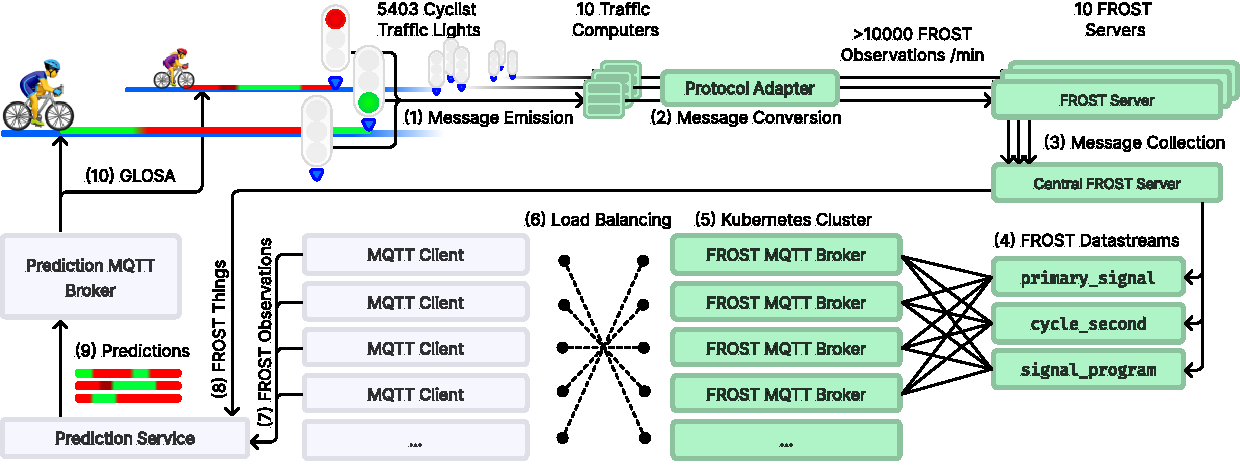
\includegraphics[width=\linewidth]{images/traffic-light-data-infrastructure.pdf}
\caption{Designed traffic light data adapter for Hamburg's Traffic Lights Data platform.}
\label{fig:traffic-light-data-infrastructure}
\end{figure}

It is crucial to understand the type of information provided by the centralized data broker. As mentioned previously, the Traffic Light Data broker does not directly provide SPaT messages, and also no residual time until the next phase change. Instead, the traffic light state messages are provided as observations of the external traffic light state. Specifically, the state messages are provided in the OGC SensorThings\footnote{\url{https://www.ogc.org/standard/sensorthings/}} "Observation" format. Each time the signal changes its color, switches to another program, or restarts a cycle, an Observation is generated and distributed on a corresponding information channel via an MQTT broker. The prediction algorithm has to ingest this data and generate a prediction of the future states.

Until the traffic light state messages arrive at the prediction service, they are translated and shifted multiple times between various data brokers. \Cref{fig:traffic-light-data-infrastructure} highlights Hamburg's data pipeline. First, the state messages are sent in a controller-specific format, such as OCIT\footnote{\url{https://www.ocit.org/de/ocit/schnittstellen/}}, to one of ten traffic computers (1). Then, the messages are converted to Observations (2) and sent to a corresponding SensorThings server. From there, a centralized SensorThings server collects all Observations (3), which are associated with a specific type of "Datastream" encapsulating the type of Observation: \texttt{primary\_signal} for traffic light color, \texttt{cycle\_second} for cycle timing, and \texttt{signal\_program} for program change (4). Finally, the messages are redistributed across an autoscaled cluster of SensorThings MQTT brokers (5). 

From there, the prediction service connects to the broker endpoint to ingest all Observation messages. To reduce the load on each individual MQTT broker, the prediction service utilizes multiple MQTT clients with individual TCP connections (6). The collected Observations (7) are combined, knowing which Observation is associated with which Datastream and which traffic light is represented by a "Thing" (8). This allows the prediction service to record the traffic light history and employ the probabilistic prediction method proposed by Pape (2012) \cite{pape_untersuchung_2012} and Protschky et al. (2014) \cite{protschky_extensive_2014, protschky_adaptive_2014} (9). Every 60 seconds, a new prediction of 180 seconds into the future is generated for each traffic light and distributed to the smartphone app via MQTT (10). Each smartphone app is subscribed to the MQTT topic of the upcoming traffic light, meaning that predictions are automatically updated on the client side.

\begin{figure}[t]
\centering
\includegraphics[width=\linewidth]{images/monitoring-screenshot.png}
\caption{Screenshot of the developed monitoring solution. The dashboard displays the current spatial availability and quality of predictions, as well as a timeline for the ingress data and the prediction quality.}
\label{fig:monitoring-screenshot}
\end{figure}

Each time a state message is shifted along the presented chain of information, it introduces a delay and a possible point of failure. As a consequence, the prediction service must be robust against delayed or missing state messages. However, these issues are not evenly distributed across all traffic lights. They may arise in specific areas in the city or from time to time. Thus, it is also important to monitor this behavior and identify and address systematic issues in the traffic light data infrastructure. As a foundation, as shown in \Cref{fig:monitoring-screenshot}, a monitoring system was implemented that highlights data outages across the city and along a timeline.

In addition to these coarse-grained methods, another error-detection is implemented that detects missing state messages for traffic lights. The designed detection makes use of the shifting pattern red-redamber-green-amber and red-green. Transitions between phases are checked against these allowed transitions. If an illegal transition occurs, the currently recorded cycle is discarded. This makes use of the probabilistic prediction method's robustness against missing cycles.

\begin{figure}[htbp]
\centering
\includegraphics[width=\linewidth]{images/home-view-prediction-quality.png}
\caption{Prediction quality visualized in the GLOSA app for enhanced explainability.}
\label{fig:home-view-prediction-quality}
\end{figure}

Not all traffic lights in Hamburg are available for prediction. Those who are available may occasionally lose data, which error detection can partially address. Another important factor, however, is the user's perspective on the data availability. Since a degraded prediction availability will also negatively impact usability, some ideas must be found that mitigate potential disappointments on the user side. One idea implemented in the GLOSA app is increasing the explainability of the prediction system. The existing monitoring infrastructure is extended such that users can also access information about the current availability. Through the app, users can inform themselves about the current percentage of available predictions and the spatial distribution of good and bad predictions on the map. The resulting user interface shown in \Cref{fig:home-view-prediction-quality} is intended to allow users to identify faults at an early stage and then switch to an alternative app, avoiding frustration caused by missing or incorrect predictions.

\subsection{Adaptivity Analysis} 

The chosen probabilistic prediction method assumes that the green phases should roughly align with each other across the recorded cycles. Depending on the specific traffic light control program, the traffic light's deviation from a recurring base pattern may be more or less influenced by incoming traffic. Although it is clear that, as of 2023, 90.7\% of traffic lights in Hamburg \textit{can} adapt to inbound traffic, it is unclear how pronounced this behavior is. To fill this knowledge gap, we can directly measure the traffic adaptivity based on the same data provided by the SensorThings API in Hamburg. The collected information can then be utilized to estimate how well the probabilistic method will predict the traffic lights and how it may perform in relation to other methods.

First, it must be determined which metrics are suitable for measuring characteristics of traffic adaptivity. One aspect of traffic adaptivity that can be directly measured from the recorded cycles is the shift of the green phase. We can measure the green phase's start time $g_{start}(L_j)$ and end time $g_{end}(L_j)$ in each cycle $L_j$, and calculate the shift between both:

\[ \text{Shift}(L_1, L_2) = [g_{start}(L_2) - g_{start}(L_1), g_{end}(L_2) - g_{end}(L_1)] \]

In the example given in \Cref{fig:types-of-adaptiveness}, $\text{Shift}$$(L_1, L_2)$ would be $[-2, -2]$ and $\text{Shift}$$(L_2, L_3) $$= [3, 3]$. While partially adaptive traffic lights, as highlighted in \Cref{fig:types-of-adaptiveness} are assumed to shift the green phase within the cycle, other traffic lights may only insert a green phase once a vehicle is detected. Thus, one problem of this metric is that each cycle may have different numbers of green phases. As a result, we have to discard additional green phases at the end of one cycle that are not seen in the other cycle, potentially leading to some discarded information. 

\begin{figure}[t]
    \centering
    \includegraphics[width=0.75\linewidth]{images/explanation-partially-adaptive.pdf}
    \caption{Partially adaptive traffic light switching pattern as highlighted by Otto et al. (2023) \cite{otto_framework_2023}}\label{fig:types-of-adaptiveness}
\end{figure}

To account for this loss of information, we calculate another metric to capture the cycles that are not fully considered through the Shift metric. This metric indirectly measures the deviation by the number of seconds in the current cycle that deviate from the previous cycle. We name this metric "Distance" since it calculates the second-wise distance between the cycles. The Distance metric between two cycles $L_1$ and $L_2$, with the lengths $l_1$ and $l_2$ calculated as follows:

\[ \text{Distance}(L_1, L_2) =  \sum_{i=0}^{\max(l_1, l_2)-1} \left\{
\begin{array}{ll}
1 & \text{if } i \geq l_1 \text{ or } i \geq l_2 \\
1 & \text{if } L_1[i] \neq L_2[i] \\
0 & \text{otherwise}
\end{array} \right.\]

If we apply this metric to the example in \Cref{fig:types-of-adaptiveness}, we get $\text{Distance}$$(L_1, L_2)$$ = 4$ and $\text{Distance}$$(L_2, L_3)$$ = 6$. This metric captures all second-wise differences but not the directionality of the green phase shifts. This means that traffic lights expressing a "staircase" pattern, in which the green phase is shifted by a constantly increasing factor each cycle, will be measured as highly adaptive, although they express a relatively predictable pattern. As a consequence, both the Distance and Shift metrics are used in conjunction with the recorded traffic light data.

\begin{Summary}[Summary of Methods]
The designed prediction infrastructure makes use of Hamburg's centralized Traffic Light Data platform and reuses the existing probabilistic prediction method  \cite{pape_untersuchung_2012, protschky_extensive_2014, protschky_adaptive_2014} guaranteeing scalability in addition to robustness to latencies and data errors. Interoperability with platforms without the availability of intersection-controller-level predictions (as with SPaT messages) is also given since the prediction algorithm only relies on the availability of traffic light colors and cycle timing information. Additional measures are implemented that detect and discard erroneous data. Through a monitoring system the prediction quality can be analyzed and systematic issues identified. Information about the prediction availability is forwarded to the user to enhance the explainability of outages. In addition to this monitoring system, an adaptivity analysis is conducted to explore the traffic-adaptiveness of traffic lights. This adaptivity analysis reuses the traffic light data infrastructure for direct measurement of the adaptiveness instead of extrapolating on the reported number of 90.7\% adaptive traffic lights. The adaptiveness is measured with two metrics in conjunction: the Distance metric incorporating the absolute shift between traffic light cycles, and the Shift metric that measures the directionality in the traffic light switching patterns.
\end{Summary}

\section{Results}

- Die Evaluation der Prognoseinfrastruktur ist zweigeteilt: die Auswertung des Prognoseverfahrens und die Auswertung der Verkehrsadaptivität von Ampeln in Hamburg.

- Als erstes betrachten wir, wie gut das Prognosesystem im Zusammenspiel mit der Hamburger Ampeldatenplattform funktioniert, und wo mögliche Schwachstellen sind.
- Dazu schauen wir uns die räumliche Abdeckung und den Verlauf der Ampelprognosen über einen längern Zeitraum an. Die Grundlage dafür bilden die Aufgezeichneten Metriken des umgesetzten Monitoring-Systems
- Wir schauen uns den zeitlichen Verlauf der Prognoseverfügbarkeit an. Dies gibt uns Aufschlüsse darüber, an wievielen Ampeln in Hamburg Geschwindigkeitsempfehlungen zu erwarten sind, und dass dies deutlich weniger sind als gewünscht
- Um genauer nachzuvollziehen, warum die Prognoseverfügbarkeit niedriger als gewünscht ist, schauen wir auf die aufgezeichneten Metriken des umgesetzten Monitoring-Tools
- Wir identifizieren bestimmte wiederkehrende Fehlermuster, die auf systematische Fehler in der Hamburger Dateninfrastruktur hinweisen
- Gemeinsam mit den Betreibern der Datenplattform ziehen wir Rückschlüsse auf die Problemursachen und beschreiben mögliche Lösungsansätze
- Um die Skalierbarkeit des Prognosealgorithmus nochmals zu zeigen schauen wir uns noch kurz die CPU, RAM und Netzwerkauslastung des Prognosedienstes an

- Der zweite Teil der Evaluation bezieht sich auf die Untersuchung der Verkehrsadaptivität über die Echtzeitdaten
- Wir betrachten den Tag-Nacht Zyklus der Verkehrsabhängigkeit von Wochentag zu Wochentag und schauen uns an, wie stark die Grünphase der Ampeln in einem Zyklus nach vorn und hinten schwankt. Grundlage hierfür ist die entwickelte Distance metrik
- Außerdem schauen wir uns an, ob die Grünphasen tendenziell gleichverteilt innerhalb des Zyklus nach vorn oder hinten streuen, oder ob es Ampeln mit Stufenmustern gibt, bei denen die Grünphase nur nach vorn oder nur nach hinten streut
- Anhand einer Karte betrachten wir, ob die Verkehrsabhängigkeit wie erwartet immer ganze Knoten mit mehreren Ampeln betrifft, oder auch einzelne Ampeln
- Diese drei Analysen helfen uns, genauer einzuschätzen, an wie vielen Kreuzungen das gestaltete Prognoseverfahren geeignet ist

\subsection{Long-Term Study of Prediction Availability, Quality, and Scalability}

\begin{table}[b]
    \centering
    \begin{tabular}{@{}l|ccccccccc|r@{}}
        \hline
        Lane type & \multicolumn{9}{c|}{Tag according to \texttt{Thing/properties/laneType}} & $\Sigma$ \\
        \hline
        Car        & $\blacksquare$ & $\blacksquare$ & $\blacksquare$ &   &   & $\blacksquare$ &   &   &   &  9649 \\
        Bus        &   &   & $\blacksquare$ &   &   & $\blacksquare$ & $\blacksquare$ &   & $\blacksquare$ &  1309 \\
        Bike     & $\blacksquare$ &   & $\blacksquare$ & $\blacksquare$ &   &   &   & $\blacksquare$ & $\blacksquare$ &  5477 \\
        Pedestrian &   &   &   &   & $\blacksquare$ &   &   & $\blacksquare$ &   &  6408 \\
        \hline
        $\Sigma$ (unique) & 1509 & 7077 & 217 & 3646 & 6315 & 846 & 234 & 93 & 12 & \\
        \hline
    \end{tabular}
    \caption{Number of individual traffic lights (connections) in the Traffic Lights Data platform, as of Dec 4, 2023.}
    \label{tab:tld-number-of-things}
\end{table}

- Bei der Betrachtung des zeitlichen Verlauf der Prognose muss zunächst beachtet werden: Die Anzahl Ampeln in der Traffic Lights Data plattform nimmt stetig zu
- Wir können die ID der individuellen Ampeln (connections) nutzen um die Anzahl Kreuzungen zu bestimmen, wie z.B. \texttt{353\_12} für Kreuzungsknoten 353 und Connection 12
- Siehe \Cref{tab:tld-number-of-things}: Zum Stand Dezember 2023 befanden sich 19951 ampeln (connections) verteilt über 791 kreuzungsknoten im System. Dies ergibt eine Abdeckung von 45.7\% (von 1731) der signalisierten Kreuzungen
- Bei der Sichtung der Ampeln wurden zwei kleine Fehler festgestellt:
- Bei einer der Ampeln (132\_22) wurde ein doppelter cycle\_second Datastream festgestellt
- Außerdem wurden bei den 2 Connections 240\_1 und 240\_2 fälschlicherweise der laneType "16371" angegeben, der eigentlich die Meldepunktnummer darstellt. Diese sind in \Cref{tab:tld-number-of-things} nicht mit aufgeführt, da sie nicht zugeordnet werden können
- Beide Probleme konnten durch Kommunikation mit den Betreibern auf Fehler in der Dateneinpflegung zurückgeführt werden. Die Behebung der Fehler wurde eingeleitet.

- Stand Dec 4, 2023 sind von den 19951 Ampeln 5477 für die Benutzung durch Radfahrer markiert und damit relevant für unser bike-GLOSA System. Auch eine Mischbenutzung durch ÖPNV, Fußgänger, und Autos zusammen mit Fahrrädern ist hierbei mit einbezogen
- Die aufgezeichneten Daten für diese Ampeln ergeben, gemessen über einen Zeitraum von 365 Tagen (Dec 4, 2022 -- Dec 4, 2023), im Durchschnitt 8532 primary\_signal Observations, 3318 cycle\_second Observations, und 27.7 program\_change Observations pro Minute die über MQTT empfangen und verarbeitet werden
- In dieser Zeit war der Prediction Service 75h wegen geplanten Wartungsarbeiten oder technischen Problemen offline und 8680h online (99.14\% uptime). Für 5h ist der Status unklar, da die gesamte VM oder nur das Monitoring offline war. Mit 80h angenommer Downtime kommen wir auf 99.08\% uptime. Daher sollte beachtet werden, wenn die nachfolgenden Metriken interpretiert werden, dass nicht 100\% des Zeitraums abgedeckt sind

\begin{figure}[t]
    \centering
    \includegraphics[width=\linewidth]{images/monitoring-availability.pdf}
    \caption{Long-term development of prediction availability.}\label{fig:monitoring-availability}
\end{figure}

- Den Langzeit-Datenverlauf sowie die Prognoseverfügbarkeit ist in  \Cref{fig:monitoring-availability} gezeigt.
- Die Prognoseverfügbarkeit errechnet sich hierbei einfach aus der Anzahl Prognosen für Ampeln, die minütlich vom Prognosedienst erzeugt werden, durch die Anzahl verfügbarer Connections
- Im oberen Teil der Abbildung sehen wir, dass die Prognoseverfügbarkeit sich im Normalfall zwischen 40\% und 80\% bewegt. 100\% werden nie erreicht.
- Die Prognoseverfügbarkeit schwankt im Tagesverlauf, aber auch im längeren Verlauf der Aufzeichnung
- Betrachten wir den längeren Verlauf, sehen wir, dass nach einer initialen Zeit mit relativ stabiler Prognoseverfügbarkeit im Sommer 2023 vermehrt Einbrüche zu beobachten sind. Diese stabilisieren sich gegen Oktober 2023 wieder, kommen aber nicht wieder auf das Niveau vom Frühjahr 2023.
- Die Einbrüche im Sommer 2023 sind hauptsächlich dadurch zu erklären, dass während dieser Zeit vermehrt Wartungsarbeiten am Traffic Lights Data System stattfanden. Es wurden wiederholt Updates durchgeführt, die zu einer Verschlechterung der Datensituation führten

- An den Tagen um den 11. Juli 2023 (1) kam es beispielsweise zu dem Problem, dass alle Observations doppelt geschickt wurden. Dies hatte zur Folge, dass die Prognoseverfügbarkeit für diesen Zeitraum fast auf 0\% zurück ging. Dies ist bisher der größte beobachtete Einbruch. Eine Vermutung, warum hierbei die Prognoseverfügbarkeit so stark einbrach, ist, dass die Duplikate der Nachrichten von einem gespiegelten System mit anderer Latenz kamen, und somit zu einer unterschiedlichen Zeit als die originale eintrafen.
- An den Tagen um den 23. November 2023 (2) wurde ein Feature für den Prognosedienst getestet, welches nicht funktionierende Ampeln aus dem System ausschließt. Daher ist die relative Verfügbarkeit in dieser Zeit kurz gestiegen trotz fallender Anzahl von Observations. 
- Abgesehen von diesen zwei besonderen Situationen ist aber klar sichtbar, dass die Prognoseverfügbarkeit stark mit der absoluten Anzahl der Nachrichten korelliert
- Ebenfalls ungeklärt ist der Abfall der signal\_program observations im Dezember 2022. Ob zum jetzigen Zeitpunkt nur ein Bruchteil der eigentlichen Programm-Observations kommen, oder im Dezember 2022 zu viele dieser Observations gesendet wurden, kann mangels einer Ground-Truth und einer Aufzeichnung genauerer Metriken für diesen Zeitraum nicht nachvollzogen werden

- Was bei der Betrachtung der Prognoseverfügbarkeit in \Cref{fig:monitoring-availability} nicht eingerechnet ist, ist die Qualität der Prognose. 
- Ein Teil der Prognosen wird zwar erstellt, hat jedoch eine niedrige Qualität. Da bei einer Prognosequalität niedriger als 50\% keine Geschwindigkeitsempfehlung dargestellt wird, ist die tatsächliche Verfügbarkeit von Geschwindigkeitsempfehlungen immer niedriger als die Prognoseverfügbarkeit

\begin{figure}[t]
    \centering
    \includegraphics[width=\linewidth]{images/monitoring-long-term-study.pdf}
    \caption{Long-term development of prediction quality.}\label{fig:monitoring-long-term-study}
\end{figure}

- Die Qualität der Prognosen ist in \Cref{fig:monitoring-long-term-study} genauer dargestellt
- Die Messung der Qualität findet statt durch einen kontinuierlichen Vergleich der Prognose mit den tatsächlich eingehenden Daten
- Stimmen alle Sekunden in der Prognose mit den aktuellen Daten überein, so errechnet sich eine Prognosequalität von 100\%. Stimmt keine Sekunde überein, so ergibt dies 0\% Prognosequalität. In der aktuellen Implementation des Prognoseverfahrens gibt es noch die Prognosequalität -1, die dann erzeugt wird, wenn nicht mindestens 5 Zyklen in den letzten 30 Minuten zur Validierung vorliegen. In \Cref{fig:monitoring-long-term-study} wird dies als Prognose mit Qualität 0\% gemapped 
- Im Langzeitverlauf sieht man zunächst einen ähnlichen Verlauf bei der Prognoseverfügbarkeit 100\% im Vergleich zu \Cref{fig:monitoring-availability} - sehr prägnant ist hier auch der Einbruch rund um den 11. Juli 2023 durch die duplizierten Observations, sowie die generell über den Jahresverlauf 2023 eingebrochene Verfügbarkeit

- Weiterhin sieht man, dass die Prognosequalität sehr zweigespalten ist: nur wenige Prognosen liegen im Bereich 10\% -- 90\% Qualität - wenn man die Prognosequalität als Genauigkeitsmetrik interpretiert, scheinen die meisten Prognosen also auf wenige Sekunden genau zu sein
- Was man jedoch auch sieht sind die vermehrten Prognosen bei 0\% Qualität Seit ca. Juli 2023. 
- Da der Prognosealgorithmus nur dann eine Prognose erzeugt, wenn bereits zu einem früheren Zeitpunkt Echtzeitdaten der Ampel vorhanden waren, lässt dies auf zwischenzeitliche Datenausfälle schließen
- Diese Datenausfälle können normal sein, beispielsweise bei der nächtlichen Abschaltung einer Ampel, oder auch nicht gewollt, wenn dies außerplanmäßig und irregular geschieht. Letzteres würde dann auf ein systematisches Problem in der Dateninfrastruktur hindeuten
- Also lohnt es sich, nochmal einen genaueren Blick auf die Datenausfälle zu richten

\begin{figure}[htbp]
    \centering
    \begin{tabular}{@{}cp{5cm}c@{}}
    (a) 6:00 UTC & & (b) 7:00 UTC\\
    \end{tabular}
    \includegraphics[width=\linewidth]{images/monitoring-before-after-failure.png}
    \caption{Before and after traffic computer failure on Oct 11, 2023. Green to red: 100\% to 0\% prediction quality. Black: no prediction, or quality -1.}\label{fig:monitoring-failure}
\end{figure}

- Ein willkürlich gewähltes Beispiel eines solchen Datenausfalls ist in \Cref{fig:monitoring-failure} gezeigt.
- Sichtbar sind hierbei zwei Arten von Problemen: Ausfälle vereinzelter Ampeln (links und rechts) und Ausfälle ganzer Stadtteile (nur rechts)
- Bei Ausfällen einzelner Ampeln 

- TEST wird dies synchronisiert?

\begin{figure}[htbp]
    \centering
    \includegraphics[width=\linewidth]{images/monitoring-failure.pdf}
    \caption{Monitored metrics during traffic computer failure on Oct 11, 2023.}\label{fig:monitoring-failure}
\end{figure}

\begin{figure}[htbp]
    \centering
    \includegraphics[width=\linewidth]{images/monitoring-7-days.pdf}
    \caption{Reoccurring traffic computer failures after 6:00 UTC.}\label{fig:monitoring-7-days}
\end{figure}

Together with the Traffic Light Data system operators (LSBG, HHVA, SWARCO), this monitoring system was utilized to identify multiple problems:

\begin{enumerate}
    \item It occasionally happens that traffic control centers need to undergo maintenance. During this period, real-time data is usually not available for a particular area of the city.
    \item During the day, the SensorThings brokers cannot keep up with the incoming number of messages. Consequently, brokers' queues fill up, leading to dropped messages.
    \item Messages from specific traffic control centers can arrive with significant delays of several minutes. This may prevent the generation of predictions for certain traffic lights, as the constraint for time criticality is violated.
    \item Some traffic lights were connected to the Traffic Lights Data platform, although their protocol is currently not supported by the protocol adapter. These traffic lights would be offline all the time.
    \item Due to construction or general changes in intersection layouts, some traffic lights would be associated with the wrong ID or not exist anymore.
\end{enumerate}

Based on the collected knowledge, these issues could be addressed accordingly. First, the platform operators were able to improve the stability of affected brokers. Then, to address issues 3--5, all traffic nodes associated with the erroneous traffic computers and erroneous traffic lights were excluded based on a list provided by the system's operators. This significantly reduces the number of available traffic lights for the prediction system but ensures that predictions are only provided for functional traffic lights.

Lösungsmöglichkeiten:
- HTTP-MQTT-Syncing (für Datenaufzeichnung zu Evaluationsteil 2 verwendet, aber für Datenaufzeichnung des Prognosesystems nicht)

- To show the effect of the improvements: rejected cycles metric

\begin{figure}
    \centering
    \includegraphics[width=\linewidth]{images/monitoring-rejected-cycles.pdf}
    \caption{Cycles rejected due to out-of-order phase sequence.}\label{fig:monitoring-rejected-cycles}
\end{figure}

\begin{figure}
    \centering
    \includegraphics[width=\linewidth]{images/monitoring-prediction-service-load.pdf}
    \caption{Cadvisor statistics for prediction service.}\label{fig:monitoring-prediction-service-load}
\end{figure}



\subsection{Study of Traffic-Adaptivity in Hamburg}

...

\section{Conclusions}
